%!TEX root = ../out/14-review-SL.tex

\begin{document}
	
\mytitle{Review}{Review}


\section{Review}

\subsection{Upper Bounds}

\begin{frame}{Kernelization: definition}

\begin{definition}
	A \alert{kernelization} for a parameterized problem $\Pi$ is a
	\textbf{polynomial time} algorithm, which, for any instance $I$ of $\Pi$ with parameter $k$,
	produces an \textbf{equivalent} instance $I'$ of $\Pi$ with parameter $k'$ such that
	$|I'| \le f(k)$ and $k'\le f(k)$ for a computable function $f$.\\
	We refer to the function $f$ as the \alert{size} of the kernel.
\end{definition}

\end{frame}

\begin{frame}
\frametitle{Main Complexity Classes}

\noindent
$\P$: class of problems that can be solved in time $n^{O(1)}$\newline
$\FPT$: class of problems that can be solved in time $f(k) \cdot n^{O(1)}$\newline
$\W[\cdot]$: parameterized intractability classes\newline
$\XP$: class of problems that can be solved in time $f(k) \cdot n^{g(k)}$ %; ``polynomial when the parameter is a constant''.
%
\slides{\bigskip}
\begin{align*}
\P \subseteq \FPT \subseteq \W[1] \subseteq \W[2] \dots \subseteq \W[P] \subseteq \XP
\end{align*}
\slides{\bigskip}

\noindent
Known: If $\FPT = \W[1]$, then the Exponential Time Hypothesis fails,
i.e. 3-\textsc{Sat} can be solved in time $2^{o(n)}$.

\end{frame}


\begin{frame}
\frametitle{Search trees}

\textbf{Recall}: A \alert{search tree} models the recursive calls of an algorithm.\\
For a $b$-way branching where the parameter $k$ decreases by $a$ at each recursive call, the number of nodes is at most $b^{k/a}\cdot (k/a+1)$.

\begin{center}
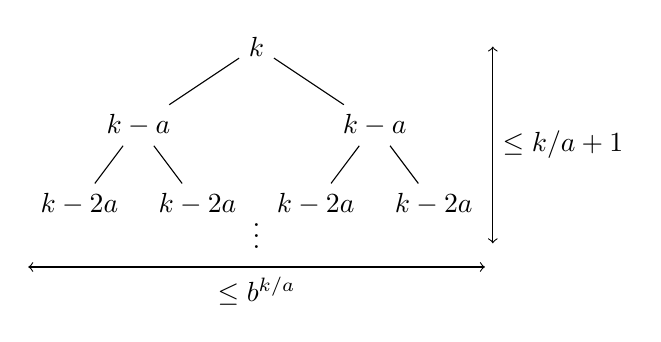
\begin{tikzpicture}
[level distance=10mm,
level 1/.style={sibling distance=30mm},
level 2/.style={sibling distance=15mm}]
\node {$k$}
child {node {$k-a$}
	child {node {$k-2a$}}
	child {node {$k-2a$}}
}
child {node {$k-a$}
	child {node {$k-2a$}}
	child {node {$k-2a$}}
};
\node at (0,-2.3) {$\vdots$};
\draw[<->] (3,0)--(3,-2.5) node[midway,right] {$\le k/a+1$};
\draw[<->] (-2.9,-2.8)--(2.9,-2.8) node[midway,below] {$\le b^{k/a}$};
\end{tikzpicture}
\end{center}

If $k/a$ and $b$ are upper bounded by a function of $k$,
and the time spent at each node is \FPT\ (typically, polynomial),
then we get an \FPT\ running time.

\end{frame}

%\begin{frame}
% \frametitle{Dynamic Programming across Subsets}
% 
% \begin{itemize}
%	\item very general technique
%	\item uses solutions of subproblems
%	\item typically stored in a table of exponential size
% \end{itemize}
%
%\end{frame}

\begin{frame}
 \frametitle{Measure \& Conquer}

\begin{lemma}[Measure \& Conquer Lemma]
Let
\begin{itemize}
 \item $A$ be a branching algorithm
 \item $c \ge 0$ be a constant, and
 \item $\mu(\cdot), \eta(\cdot)$ be two measures
 for the instances of $A$,
\end{itemize}
such that
on input $I$, $A$ calls itself recursively on instances $I_1,\ldots,I_k$, but, besides the recursive calls, uses time $\cO(|I|^c)$, such that
% weights $w_e$, $w_h$, and $w_1, w_2, \ldots, w_6$ defining measure~$\mu$,
\begin{align}
(\forall i) \quad \eta(I_i) & \leq \eta(I)-1 \text{, and}  \label{eq:masize}
  \\
2^{\mu(I_1)} + \ldots + 2^{\mu(I_k)} & \leq 2^{\mu(I)} . \label{eq:magain}
\end{align}
Then $A$ solves any instance $I$
in time $\cO(\eta(I)^{c+1}) \cdot 2^{\mu(I)}$.
\end{lemma}

\end{frame}

%\begin{frame}{Inclusion-Exclusion}
%
%\begin{theorem}[IE-theorem -- intersection version]
% Let $U=A_0$ be a finite set, and let $A_1,\dots,A_k\subseteq U$.
% \begin{align*}
%  \left|\bigcap_{i\in \{1,\dots,k\}} A_i \right| = \sum_{J\subseteq \{1,\dots,k\}} (-1)^{|J|} \left| \bigcap_{i\in J} \overline{A_i} \right|,
% \end{align*}
% where $\overline{A_i} = U\setminus A_i$ and $\bigcap_{i\in \emptyset} = U$. 
%\end{theorem}
%
% \begin{theorem}
%  The number of covers with $k$ sets and the number of ordered partitions with $k$ sets of a set system $(V,H)$ can be computed in polynomial space and
%  \begin{enumerate}
%   \item $O^*(2^n|H|)$ time if $H$ can be enumerated in $O^*(|H|)$ time and poly space,
%   \item $O^*(3^n)$ time if membership in $H$ can be decided in polynomial time, and
%   \item $\sum_{j=0}^n \binom{n}{j} T_{H}(j)$ time if there is a $T_H(j)$ time poly space algorithm to count for any $W\subseteq V$ with $|W|=j$ the number of sets $S \in H$ st.\ $S\cap W = \emptyset$.
%  \end{enumerate}
% \end{theorem}
%\end{frame}


\begin{frame}[label=treedecomp,shrink=2]
  \frametitle{Tree decompositions (by example)}

  \begin{itemize}
  \item A graph $G$

\begin{tikzpicture}[yscale=.5]

 \draw[thick] 
    (0,3) node[vertex,label=left:$a$] (a) {}
    (1,4) node[vertex,label=above:$b$] (b) {}
    (2,3) node[vertex,label=above:$c$] (c) {}
    (3,3) node[vertex,label=above:$d$] (d) {}
    (2,1) node[vertex,label=left:$e$] (e) {};
 \draw[thick] 
    (3,1) node[vertex,label=below:$\textcolor{red}{f}$] (f) {};
 \draw[thick] 
    (4,2) node[vertex,label=above:$h$] (h) {}
    (4,0) node[vertex,label=right:$g$] (g) {}
    (5,2) node[vertex,label=above:$i$] (i) {}
    (6,3) node[vertex,label=right:$j$] (j) {}
    (6,1) node[vertex,label=right:$k$] (k) {}

(b)--(c) (a)--(c) (e)--(f) (c)--(d) (f)--(g) (f)--(h) (c)--(d)
(c)--(e) (d)--(h) (f)--(h)--(i)--(j) (i)--(k) ;
 \draw[very thick,color=green!50!black] (a)--(b);

\end{tikzpicture}


\item A \emph{tree decomposition} of $G$

  \begin{tikzpicture}[xscale=1.8]

    \draw[thick,ellipse]
     (-0.5,0) node[draw] (abc) {$\textcolor{green!50!black}{a},\textcolor{green!50!black}{b},c$};
    \draw[thick,ellipse]
     (1.75,0) node[draw] (def) {$d,e,\textcolor{red}{f}$}
     (3,0) node[draw] (dfh) {$d,\textcolor{red}{f},h$}
     (1.75,-1) node[draw] (fg) {$\textcolor{red}{f},g$};
    \draw[thick,ellipse]
     (0.5,0) node[draw] (cde) {$c,d,e$}
     (4,0) node[draw] (hi) {$h,i$}
     (5,1) node[draw] (ij) {$i,j$} 
     (5,-1) node[draw] (ik) {$i,k$}
     (abc)--(cde)--(def)--(dfh)--(hi)--(ij) (hi)--(ik) (def)--(fg)

;
  \end{tikzpicture}
  
  {Conditions:} 
  {\textcolor{green!50!black}{covering}}
  {and \textcolor{red}{connectedness.}}

  \end{itemize}
\end{frame}

%\begin{frame}
%	\frametitle{Iterative Compression}
%	
%	\noindent
%	For a minimization problem:
%	\begin{itemize}
%		\item \textbf{Compression step:} Given a solution of size $k+1$, compress it to a solution of size $k$ or
%		prove that there is no solution of size $k$
%		\item \textbf{Iteration step:} Incrementally build a solution to the given instance by deriving solutions for
%		larger and larger subinstances
%	\end{itemize}
%	\medskip
%	\begin{itemize}
%		\item Often, we can get a solution of size $k+1$ with only a polynomial overhead
%	\end{itemize}
%			
%\end{frame}


\begin{frame}
 \frametitle{Randomized algorithms}
 
 Solution intersects a linear number of edges:
 \begin{itemize}
 	\item Sampling vertices with probability proportional to their degree gives good success probability if the set of vertices we try to find has large intersection with the edges of the graph.
 \end{itemize}
 
 Color Coding:
 \begin{lemma}
  Let $X\subseteq U$ be a subset of size $k$ of a ground set $U$.\\
  Let $\chi: U\rightarrow \{1,\dots,k\}$ be a random coloring of $U$.\\
  The probability that the elements of $X$ are colored with pairwise distinct colors is $\ge e^k$.  
 \end{lemma}

 Monotone Local Search:
 \begin{itemize}
	\item For many subset problems a $O^*(c^k)$ algorithm for finding a solution of size $k$ can be turned into a randomized algorithm finding an optimal solution in time $O^*((2-1/c)^n)$.
\end{itemize}

\end{frame}

\begin{frame}
	\frametitle{Quantum algorithms}
	
	Many branching algorithms and randomized algorithms for NP-complete problems get a quadratic speedup on quantum computers.

\end{frame}

\begin{frame}
	\frametitle{Approximation, Heuristics and Local Search}
	
	\begin{itemize}
		\item \textbf{Approximation:} poly-time algorithm returning a feasible solution with a guarantee of the quality of the solution
		\item \textbf{Heuristics:} return a feasible solution, typically with no worst-case guarantee but good performance in practice, in a fast and simple way.
		\item \textbf{Local Search:} Given a feasible solution $S$, a local search algorithm explores whether there is an improved feasible solution $S^*$ that can be obtained from $S$ by a ``small modification''.
	\end{itemize}
	
\end{frame}

\subsection{Lower Bounds}

\begin{frame}{Reductions}

 We have seen several reductions, which, for an instance $(I,k)$ of a problem $\Pi$, produce an equivalent instance $I'$ of a problem $\Pi'$.
 
 {\small
 \begin{tabular}{p{0.22 \textwidth} c c p{0.2 \textwidth} p{0.16 \textwidth}}
  & time & parameter & special features & used for\\ \hline
  kernelization & \poly & $k'\le g(k)$ & $|I'|\le g(k)$\newline $\Pi = \Pi'$ & $g(k)$-kernels\\
  parameterized reduction & \FPT & $k'\le g(k)$ & & $\W[\cdot]$-hardness\\
%  OR-composition & \poly & $k'\le \poly(k)$ & $\Pi =$ OR($\Pi'$) & Kernel LBs\\
%  AND-composition & \poly & $k'\le \poly(k)$ & $\Pi =$ AND($\Pi'$) & Kernel LBs\\
  (polynomial parameter transformation) & \poly & $k' \le \poly(k)$ & & (Kernel LBs)\newline (S)ETH LBs\\
  SubExponential Reduction Family & subexp($k$) & $k' \in O(k)$ & Turing reduction\newline $|I'|=|I|^{O(1)}$ & ETH LBs
 \end{tabular}
 }

\end{frame}

\section{Research in Parameterized and Exact Computation}

\begin{frame}
 \frametitle{News}
 
 \begin{itemize}
  \item Recently solved open problems from \cite{DowneyF13}
  \begin{itemize}
  	\item \textsc{Biclique} is $\W[1]$-hard \cite{Lin18}
  	\item \textsc{Short Generalized Hex} is $\W[1]$-complete \cite{BonnetGLRS17}
  	\item Determining the winner of a \textsc{Parity Game} is \FPT\ in the number of values \cite{CaludeJKL017}
  \end{itemize}
  \item research focii
  \begin{itemize}
   \item enumeration algorithms and combinatorial bounds
   \item randomized algorithms
   \item treewidth: computation, bounds %on the treewidth of grid or planar subgraphs / minors
   \item bidimensionality
   \item bottom-up: improving the quality of subroutines of heuristics
   \item (S)ETH widely used now, also for poly-time lower bounds
   %\item quests for multivariate algorithms, lower bounds for Turing kernels
   \item \FPT-approximation algorithms, lossy kernels
   \item general-purpose ``modeling'' problems: SAT, CSP, ILP, Integer Quadratic Programming
   \item backdoors
   \item parameterized algorithms in AI, computational social choice, computational biology, etc.
  \end{itemize}
 \end{itemize}

\end{frame}

\begin{frame}
 \frametitle{Resources}
 
 \begin{itemize}
  \item FPT wiki: \url{http://fpt.wikidot.com}
  \item FPT newsletter: \url{http://fpt.wikidot.com/fpt-news:the-parameterized-complexity-newsletter}
  %\item Blog: \url{http://fptnews.org}
  \item cstheory stackexchange: \url{http://cstheory.stackexchange.com}
  \item FPT summer schools (include lecture slides)
  \begin{itemize}
  	\item 2017: \url{https://algo2017.ac.tuwien.ac.at/pcss/}
  	\item 2014: \url{http://fptschool.mimuw.edu.pl}
  	\item 2009: \url{http://www-sop.inria.fr/mascotte/seminaires/AGAPE/}
  \end{itemize}
  \item The Parameterized Algorithms and Computational Experiments Challenge (PACE): \url{https://pacechallenge.wordpress.com/}
 \end{itemize}

\end{frame}


\begin{frame}[t, allowframebreaks]
\slides{\frametitle{References}}
\printbibliography
\end{frame}


\end{document}
